In this work, we \cmt{focus on} in evaluating signal transmission \cmt{performance using the PRISM tool}, \cmt{explicitly} focusing on scenarios where the individual experiencing distress maintains a \cmt{stable} psychological status. 

\paragraph{Experimental setup.} We have encoded properties in CSL formalism \cmt{and utilized the} PRISM model checker v4.8 \cite{Kwiatkowska2020} is utilized \cmt{for} verification. These experiments were conducted on a \cmt{system running Ubuntu with an i7 processor and equipped with 32GB RAM}. Multiple engines can be selected (refer to documentation \cite{engines}) offering performance benefits \cmt{to} specific model structures. In addition, we have implemented the scenarios outlined in \cite{Zhu2009} to accurately model attack frequencies.

\paragraph{Artifacts.} The source code for the experiments described in this section is publicly available on a GitHub repository \cite{newcas2025}. The website provides \cmt{detailed} instructions on \cmt{for replicating} the experiments.

	    \begin{resp}{\textbf{\textit{Property 1}}}
        
        \begin{equation}
        \label{eq1}\tag{\emph{\quot{Liveness}}}
         \mathtt{ P=? [ G(\quot{\textcolor{red}{up} } \xrightarrow{} \  F \ !(\quot{\textcolor{red}{up} }))  ]} 
        \end{equation}

        
        \end{resp}
        
        \normalsize

The property \ref{eq1} evaluates the signal performance by calculating the probability of the satellite successfully collecting the signal from a beacon while facing degradation of the signal, represented by the label \emath{!\quot{\textcolor{red}{up} }}. The results indicate a 100\% probability of the system transitioning from a functioning state to a degraded state. Thus, this leads us to investigate the role of degradation features on the signal transmitted through the verification of properties \ref{eq2} and \ref{eq3}.


    \begin{figure}[!htb]
    \centering
       \begin{tabularx}{\linewidth}{ m{8cm} }
           

 \begin{minipage}[t]{12cm}
     \centering

    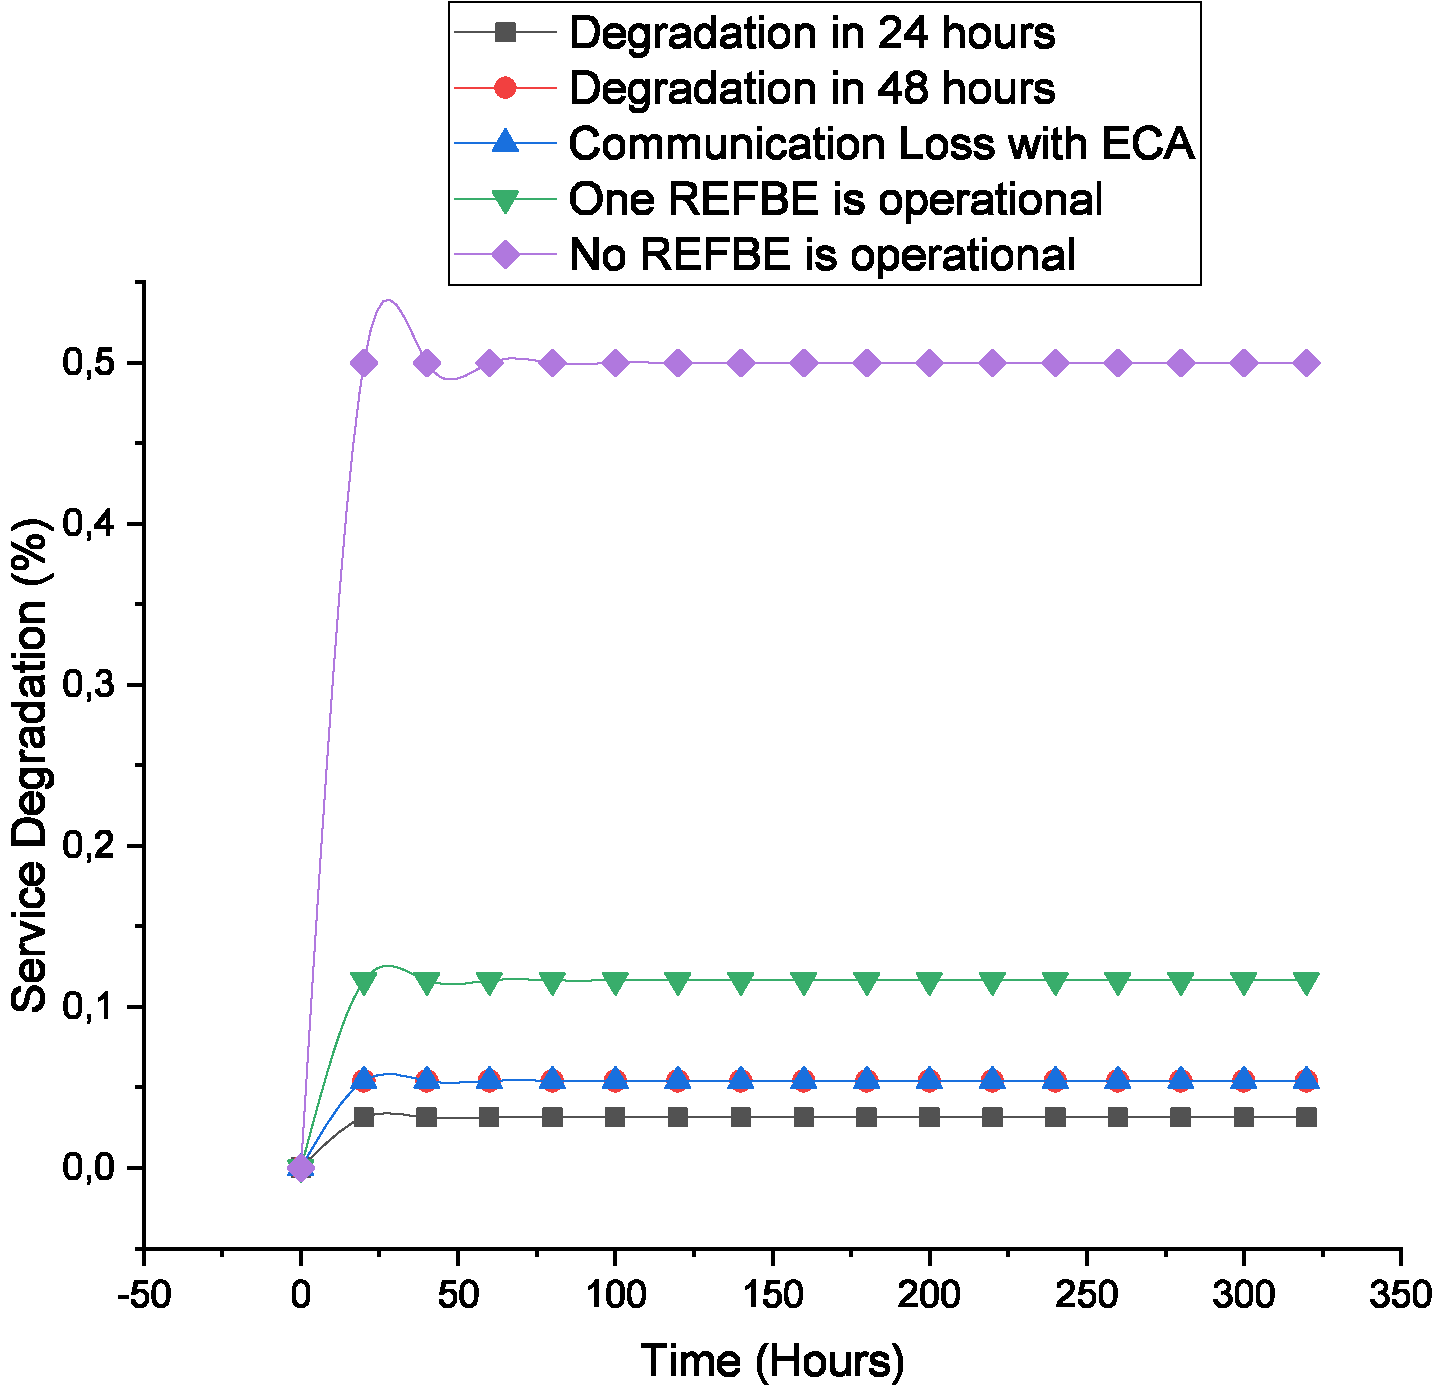
\includegraphics[width=200pt, height =180pt]{gdegraded.pdf}
    \caption{Verification of Property \ref{eq2}.}
    \label{fig:01}
   \end{minipage}
    
          \\

   \begin{minipage}[t]{12cm}
     \centering
   		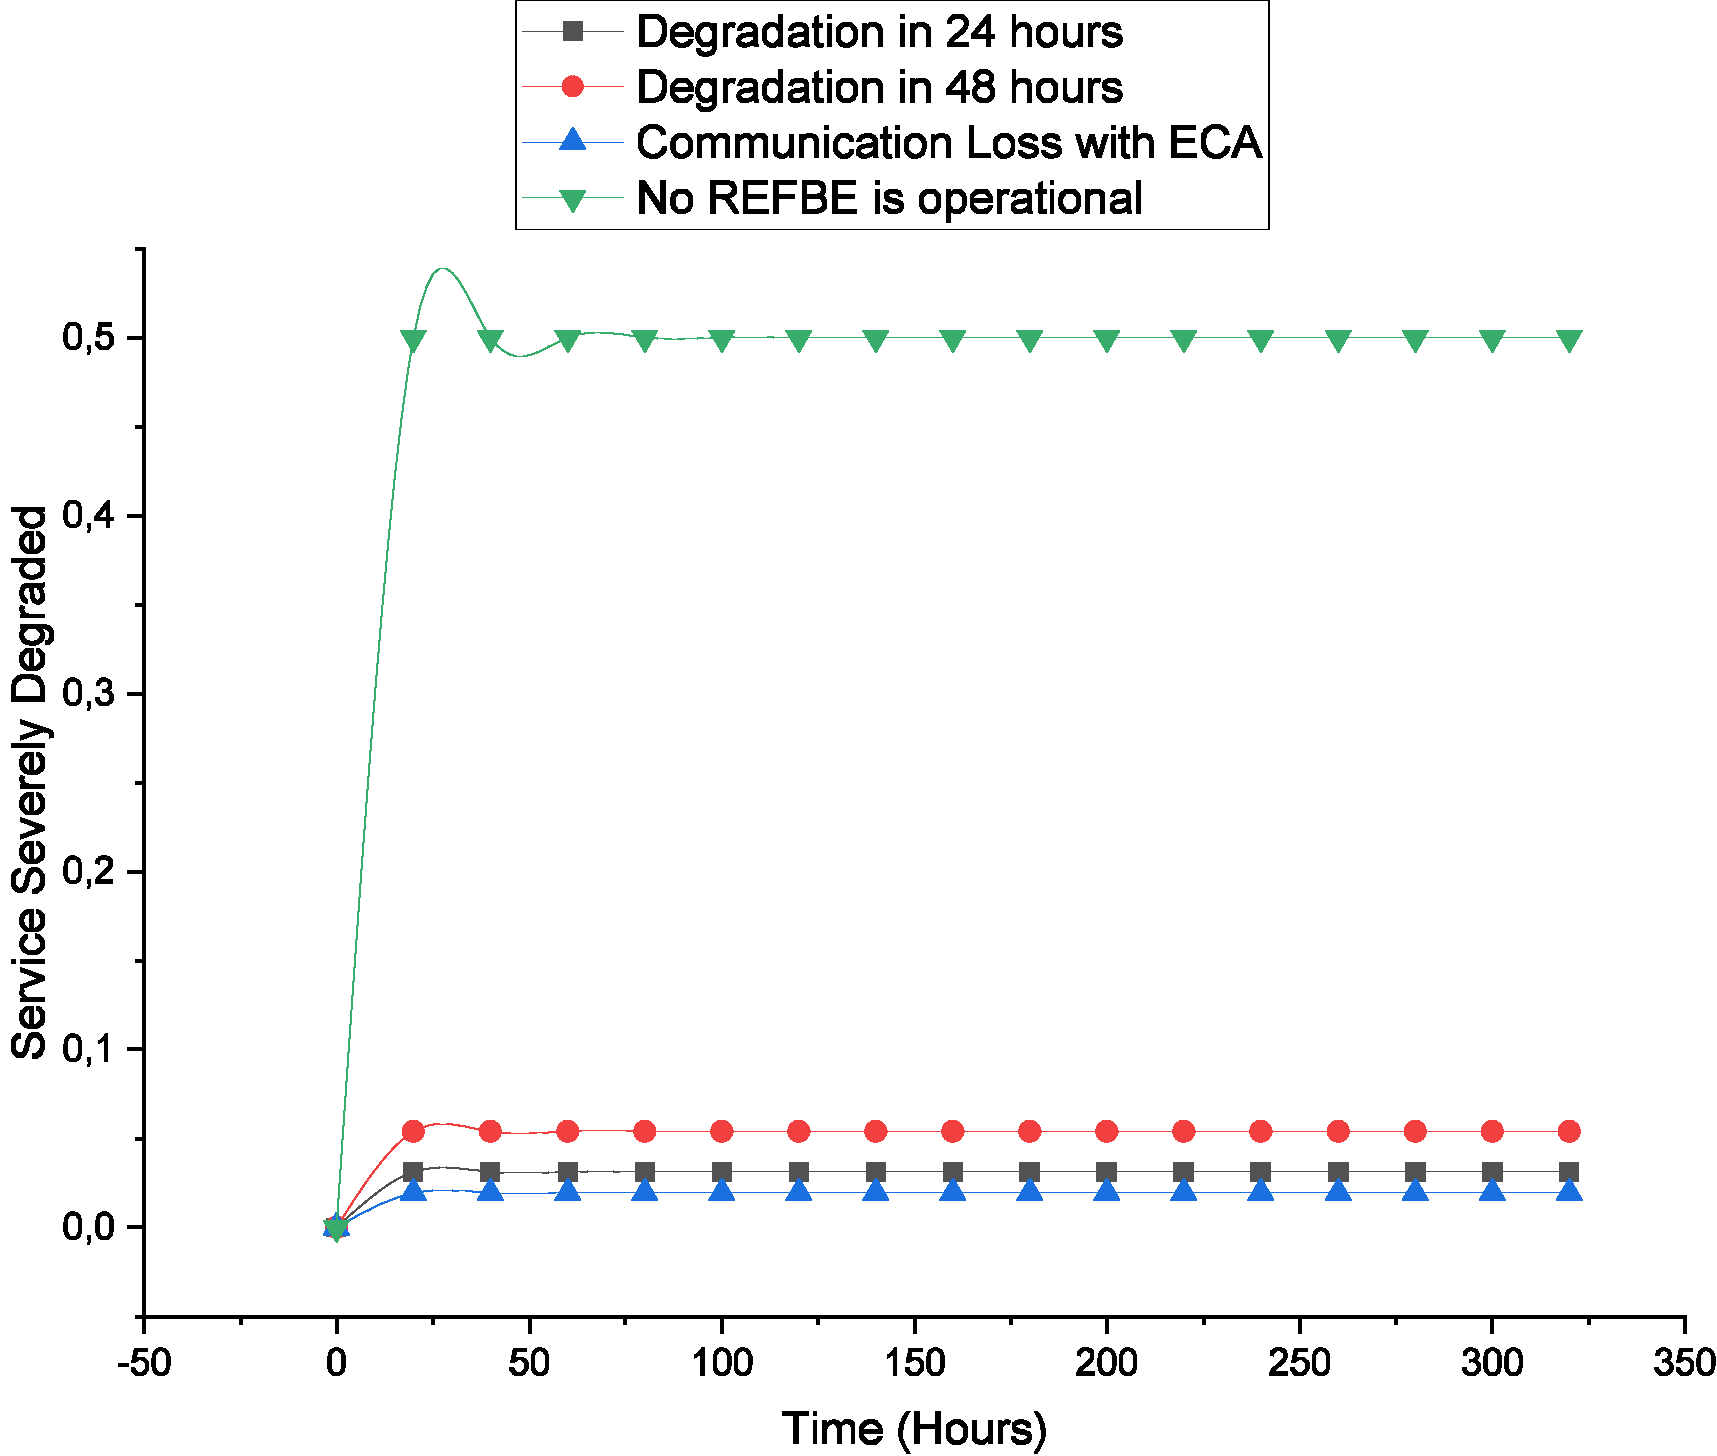
\includegraphics[width=200pt, height =180pt]{gseverlydegraded.pdf}
    \caption{Verification of Property \ref{eq3}.}
    \label{fig:02}
   \end{minipage}

               \end{tabularx}
\end{figure}


	    \begin{resp}{\textbf{\textit{Property 2}}}
        
        \begin{equation}
        \label{eq2}\tag{\emph{\quot{Degraded}}}
         \mathtt{ P=? [ (\quot{\textcolor{red}{up} }) \  U^{\leq T} \ (\quot{\textcolor{red}{Degraded} })  ]} 
        \end{equation}
        
        \end{resp}
        
        \normalsize

The property \ref{eq2} \cmt{specifies} that as time elapsed between the nominal functioning state and the degradation state increases. However, the primary distinction lies in the specific feature causing the degradation. Figure \ref{fig:01} illustrates that after 10 hours of signal transmission, the probability of degradation reaches 50\% and persists at that level for 30 calendar days due to REFBE unavailability. In contrast, internal degradation within 24 hours exhibits a low probability of 3.1\%. Notably, combining internal degradation and communication loss with ECA results in a degradation probability of 5.4\%. When only one REFBE is operational, the degradation probability reaches 11.6\%  after 20 hours of execution.


	    \begin{resp}{\textbf{\textit{Property 3}}}

        \begin{equation}
        \label{eq3}\tag{\emph{\quot{Severely Degraded}}}
         \mathtt{ P=? [ (\quot{\textcolor{red}{up} }) \  U^{\leq T} \ (\quot{\textcolor{red}{Severely\_Degraded} })  ]} 
        \end{equation}
        
        \end{resp}
        
        \normalsize


        
The property \ref{eq3} \cmt{describes} that as time elapsed between the nominal functioning state and the severe degradation state increases. However, the primary distinction lies in the specific feature causing the degradation,  \cmt{similar to the \ref{eq3} property}. Figure \ref{fig:02} illustrates that after 10 hours of signal transmission, the probability of degradation reaches 50\% and persists at that level for 30 calendar days due to REFBE unavailability. In contrast, internal degradation within 24 hours and 48 hours exhibits a low probability of 3.1\% and 5.4\%, respectively.  When communication loss with ECA, the severe degradation probability reaches 1.9\% less than the degraded mode after 20 hours of execution.

Through our analysis, we have \cmt{pinpointed} the source of service degradation within the SAR/Galileo system. \cmt{Specifically}, issues related to REFBE (Reference Beacon) monitoring of satellite performance can significantly contribute to service degradation. These \cmt{problems} can also provide maintainers with erroneous fault results, impacting maintenance activities and quality assurance.



\subsection{Discussion}
\cmt{In this study, we examined} the performance of the SAR/Galileo system, specifically focusing on degradation issues \cmt{affecting} communication between satellites and the ground stations \cmt{that assist individuals} in distress. The use case is \cmt{based on} existing documentation, and we \cmt{aim} to \cmt{evaluate} the system's \cmt{capability} to save lives by \cmt{assessing} the \cmt{communication availability of each entity involved in transmitting signals.} \cmt{Although} the signal \cmt{includes} multiple parameters not explicitly \cmt{covered} in this study, our \cmt{emphasis} remains on a high-level perspective.

The model can be extended to incorporate other factors influencing satellite signal quality, such as the impact of solar radiation, as discussed in \cite{Hoque2015,baouya2024seaa}, which can significantly affect system reliability. Furthermore, human factors should also be considered, such as an individual's \cmt{ability} to push the distress button in an \cmt{emergency promptly}. 

These results do not demonstrate the possibility that the system does not fully encompass the state of the human in terms of their reaction to danger, such as the Mean  Time To React to danger (MTTR). To address this limitation, we augment the model with a module that represents the human's status in response to a crisis in a one-month calendar. This module incorporates a formula for the rate of urgent response in line 2 of \lst{exampleinprism}: 

\begin{equation*}
\lambda_{h} = MTTR / Month 
\end{equation*}

Consequently, the model is augmented to incorporate human behavior, as illustrated in \lst{exampleinprism}. Notably, the label \quot{\textcolor{red}{\emathtt{up}}} encompasses potential human ability degradation. The PRISM command depicts a state transition from the operational mode to a degraded status for the human, upon the value of the degradation rate parameter \emath{\lambda_{h}} in line 6 of \lst{exampleinprism}. However, the correct status of the communication service depends on the system's status, which can include nominal operation, degradation, severe degradation, and the degradation of human factors in line 9.

\lstdefinestyle{framed}
{
	frame=lrb,
	mathescape,
	numbers=left,
	belowcaptionskip=-1pt,
	xleftmargin=3.11em,
	xrightmargin=0.03cm,
	framexleftmargin=3em,
	framexrightmargin=0pt,
	framextopmargin=5pt,
	framexbottommargin=5pt,
	framesep=0pt,
	rulesep=0pt,
	numbers=left,
}

\lstset{
    breaklines=true,
    style=framed,
    escapeinside={<@}{@>},
    morekeywords={void, int, public, private, class, protected, submodules, network, connections, const, init, int, bool, double, module, rewards, endrewards, endmodule,label},
    basicstyle=\small\ttfamily,
    keywordstyle=\bfseries\color{blue},
    morecomment=[f][\color{green!70!black}][0]{/*},
    morecomment=[l][\color{green!30!black}]{//},
    label=queueemodel
}

\begin{figure}[!htb]
\begin{minipage}{12cm}
\begin{lstlisting}[style=framed,
	caption=The Human Status,
 	label=exampleinprism]
const double time_to_react;
const double lambda_h=time_to_react/(30*24);

module Human_Status
 Human_Status_s : [0..3] init Operational;
 [] Human_Status_s>0 -> $\lambda_h$:(Human_Status_s'=Degraded); 
endmodule

label "up" = !degraded & !Severely_Degraded & !(Human_Status_s=Degraded);
\end{lstlisting}
\end{minipage}
\end{figure}

	    \begin{resp}{\textbf{\textit{Property 4}}}
               \begin{equation}
        \label{eq4}\tag{\quot{Rescue Service}}
         \mathtt{ P=? [ (\quot{\textcolor{red}{up} }) \  U^{\leq T} \ !(\quot{\textcolor{red}{up} })  ]} 
        \end{equation}
        \end{resp}
        
        \normalsize

        
By examining Property \ref{eq4}, which integrates human status, we observe that the system's ability to rescue a person in distress diminishes as the execution time increases, as depicted in \fig{fig:03}, regardless of the Mean Time To React (MTTR). This decrease in rescue success is attributed to the increasing likelihood of the individual experiencing a psychological state that hinders their ability to activate the distress button.

While this may seem intuitive, the verification process mathematically confirms this observation. Furthermore, the results demonstrate that the system's effectiveness depends on its capability to rescue the person in danger and crucially relies on the person's timely response to the crisis.



\begin{figure}[htbp]
     \centering
   		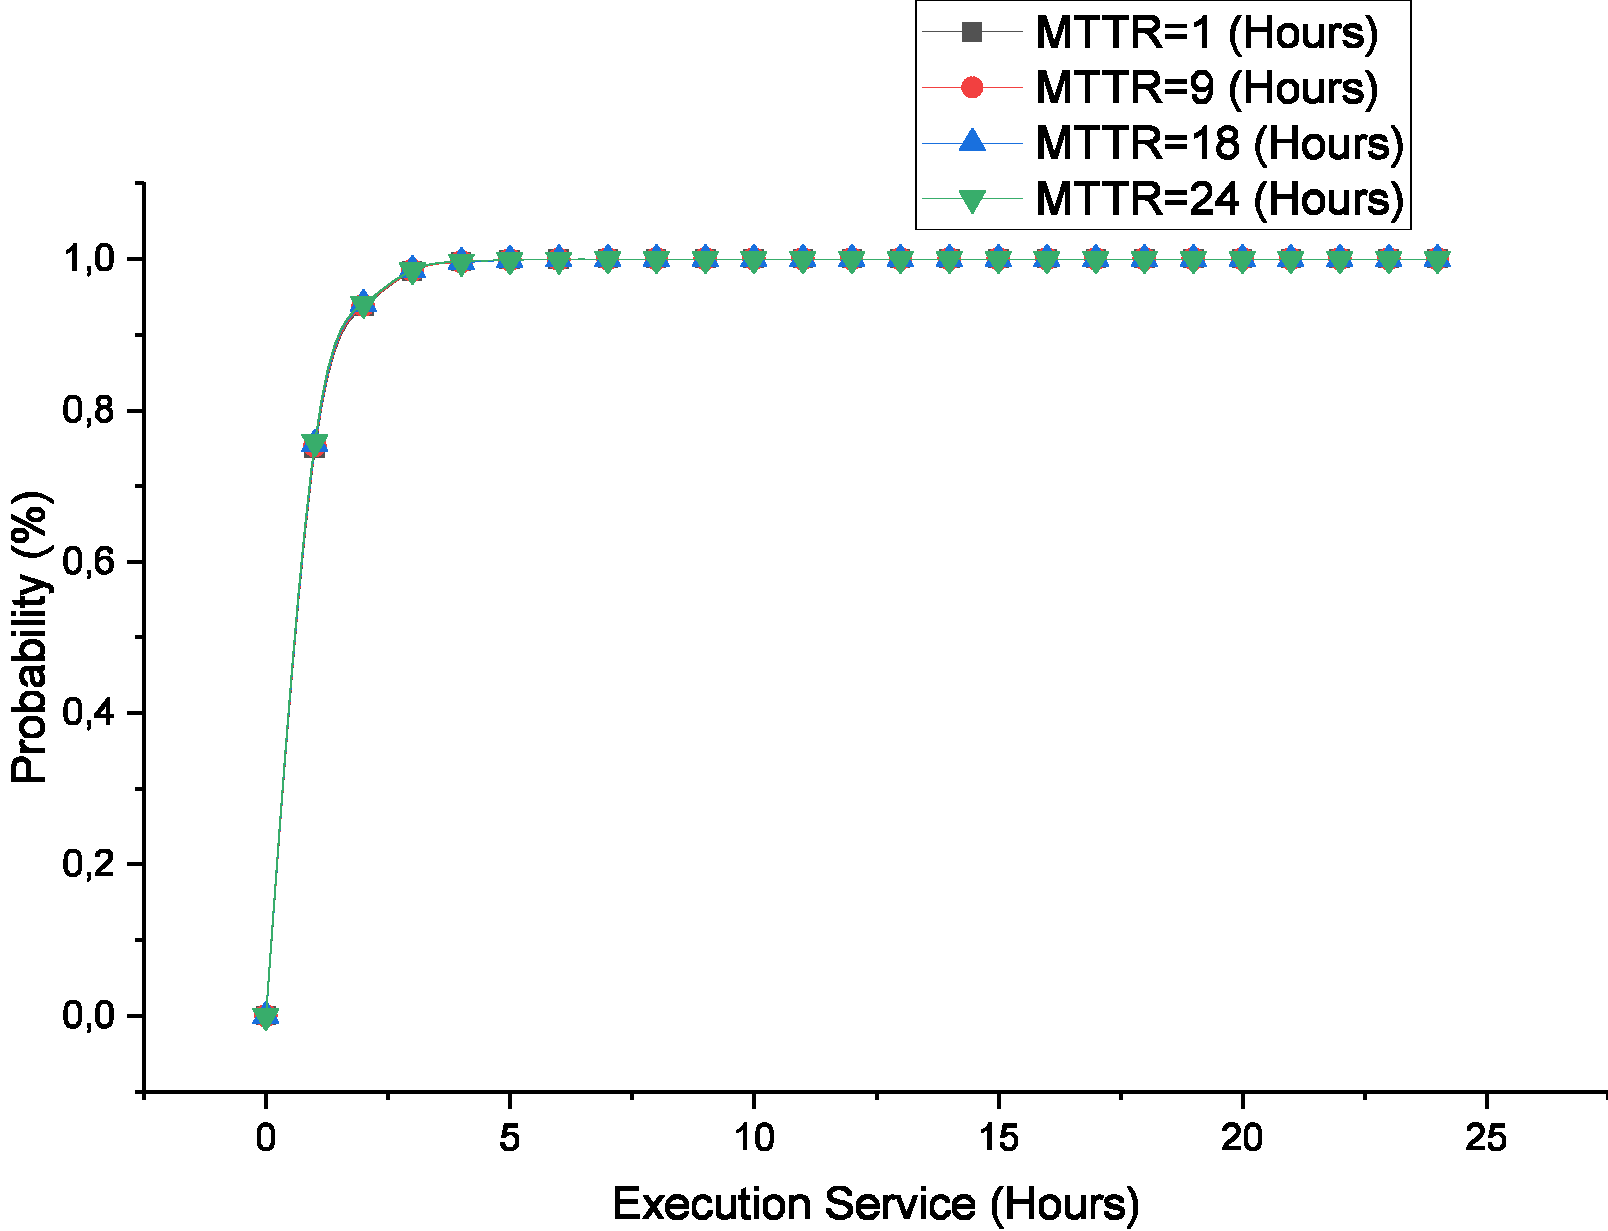
\includegraphics[width=250pt, height =180pt]{Graphh.pdf}
    \caption{Verification of Property \ref{eq4} with varied MTTR.}
    \label{fig:03}
 \end{figure} 

\subsection{Threats to validity}

This paper \cmt{focuses on specific} operational parameters of the SAR/Galileo system. \cmt{Although} other parameters \cmt{mentionned} in this SAR/Galileo documentation could \cmt{also be verified}, the PRISM model checker has limitations in supporting particular formalisms, \cmt{particulary when} incorporating satellite location and accuracy using complex data representation. These parameters necessitate high-level language specifications. \cmt{The} BIP \cite{basurigorous2011} (Behavior-Interaction-Priority) language can \cmt{effectively represent} these parameters and \cmt{facilitate} verification using a dedicated statistical model checking with SMC-BIP \cite{med2018}. 